In this section we study the performance of various jet algorithms in
combination with jet substructure variables/taggers in terms of the
identification of a boosted hadronically decaying $W$ signal. For each
jet algorithm we produce Receiver Operating Characteristic (ROC)
curves that elucidate the performance of various variables that are
capable of providing discrimination between a hadronic $W$ signal and
a QCD jet. These variables are then combined in a Boosted Decision Tree (BDT) and the performance of the resulting BDT discriminant
explored through ROC curves to understand the degree to which
variables are correlated and exploiting the same information. These
studies are repeated in different kinematic regimes, to explore both
the performance and correlations as a function of the jet boost, and
where substructure approaches may break down.

\subsection{Methodology}

These studies use the $X \rightarrow WW$ samples as signal and the XXX
samples to model the QCD background. 

Jets are reconstructed using the XXX jet algorithms described in the
previous section. The following event selection is then applied to these
samples....(presumably this will vary depending on which kinematic bin
is used, as will the actual samples used - maybe summarize in a table).

Figure~\ref{fig:pt500_basics_AKt_R08} shows
background versus signal in some basic kinematic
distributions. {\it Do we want to reweight signal kinematics to
background or vice versa? Do we want to study quarks/gluons separately?}

Go on to explain how we produce the ROC curves.

\begin{figure*}
\begin{center}
\subfigure[Leading jet
\pT]{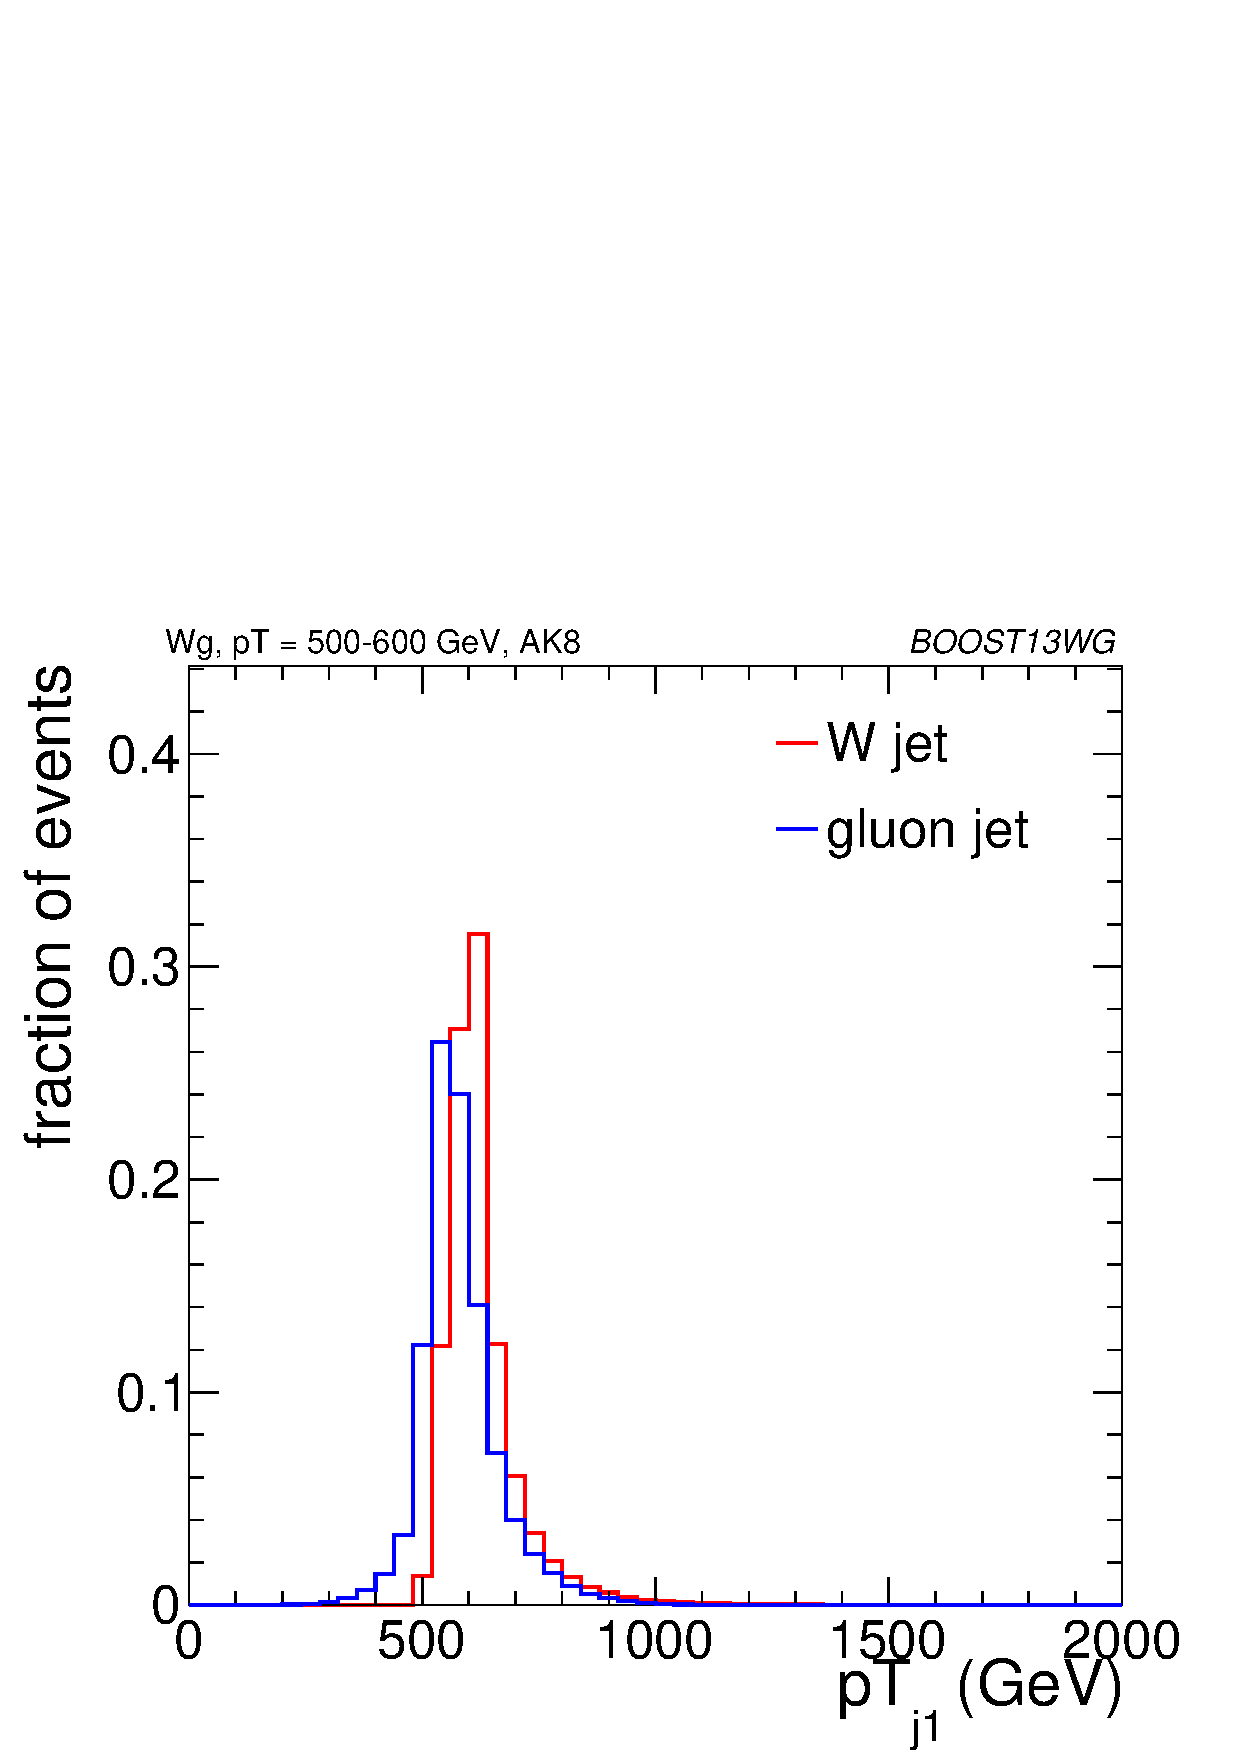
\includegraphics[width=0.48\textwidth]{./Figures/WTagging/pT500/AKtR08/jpt1.png}}
\subfigure[Sub-leading jet
\pT]{\includegraphics[width=0.48\textwidth]{./Figures/WTagging/pT500/AKtR08/jpt2.png}}
\subfigure[Leading jet
$\eta$]{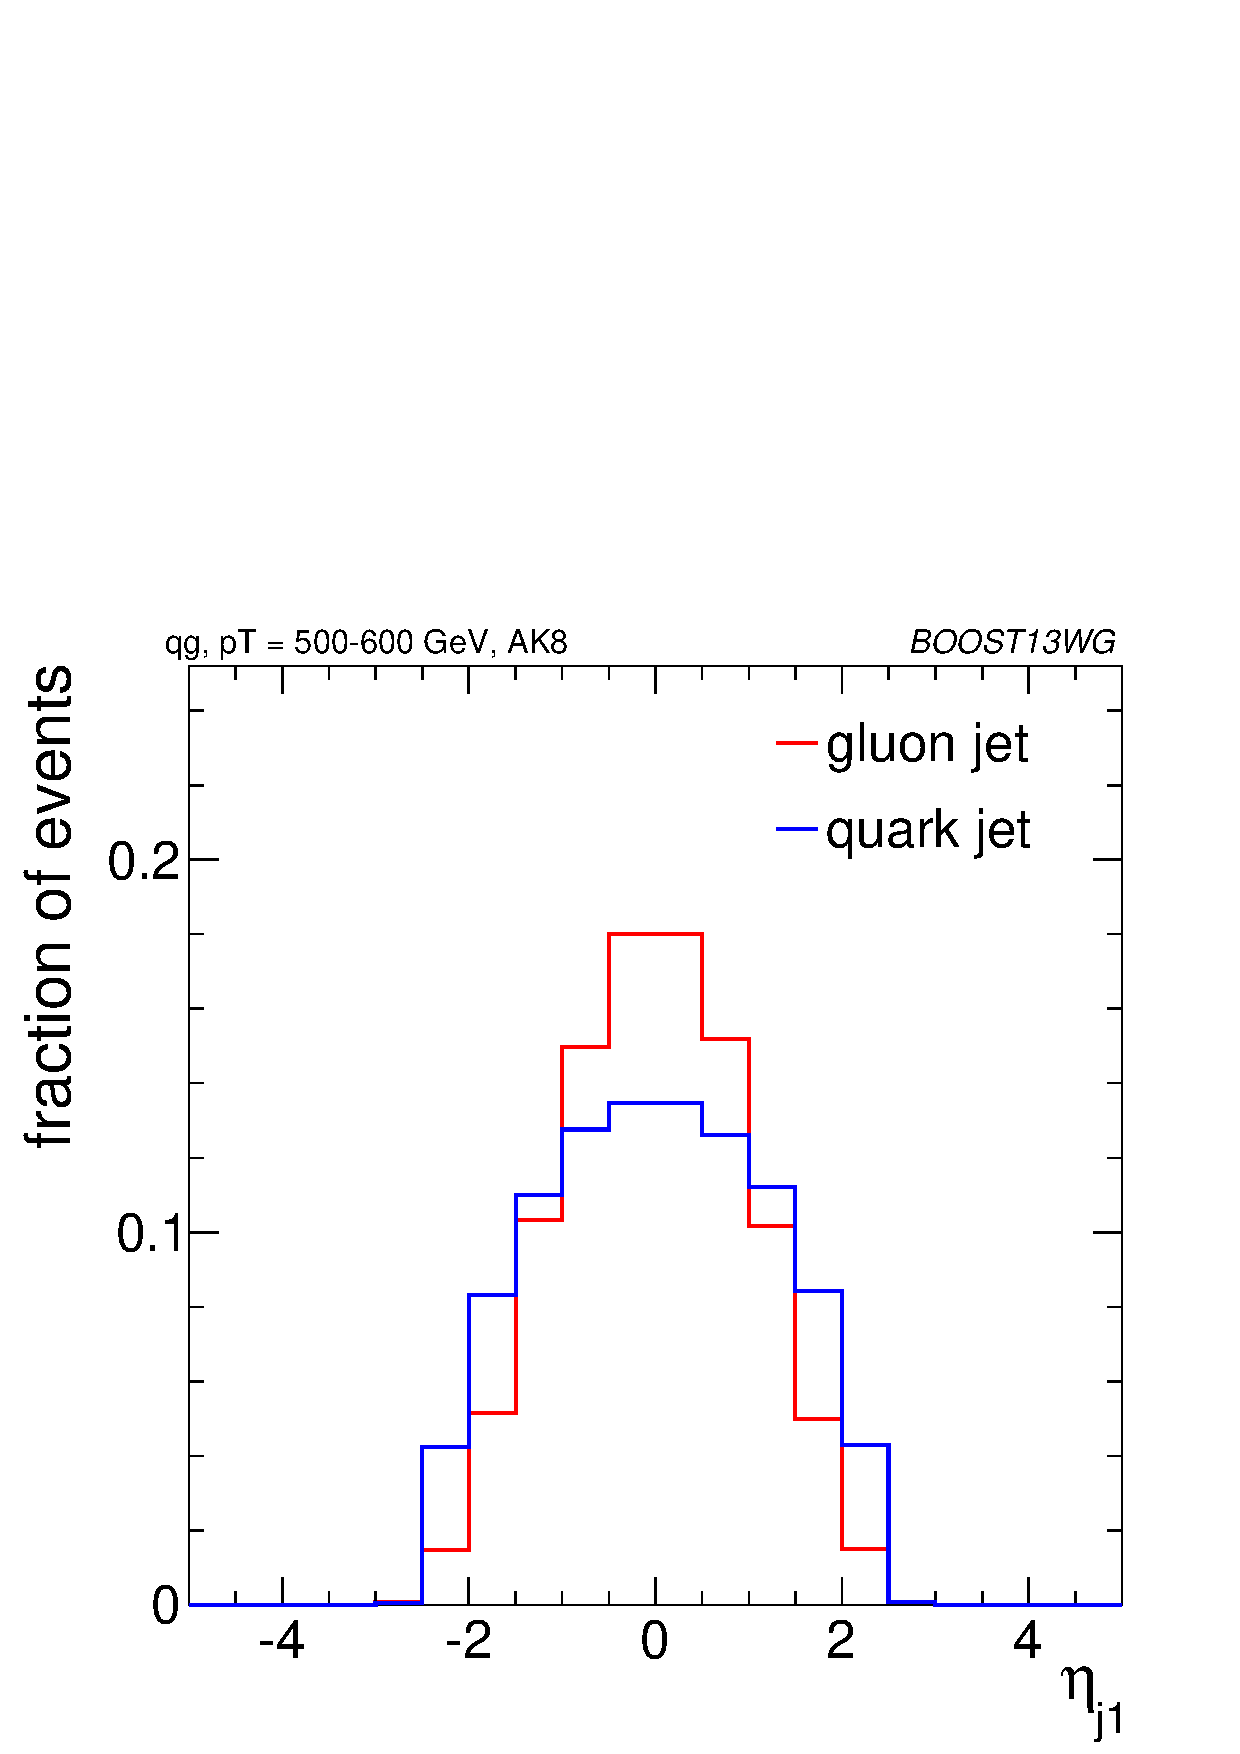
\includegraphics[width=0.48\textwidth]{./Figures/WTagging/pT500/AKtR08/jeta1.png}}
\subfigure[Sub-leading jet
$\eta$]{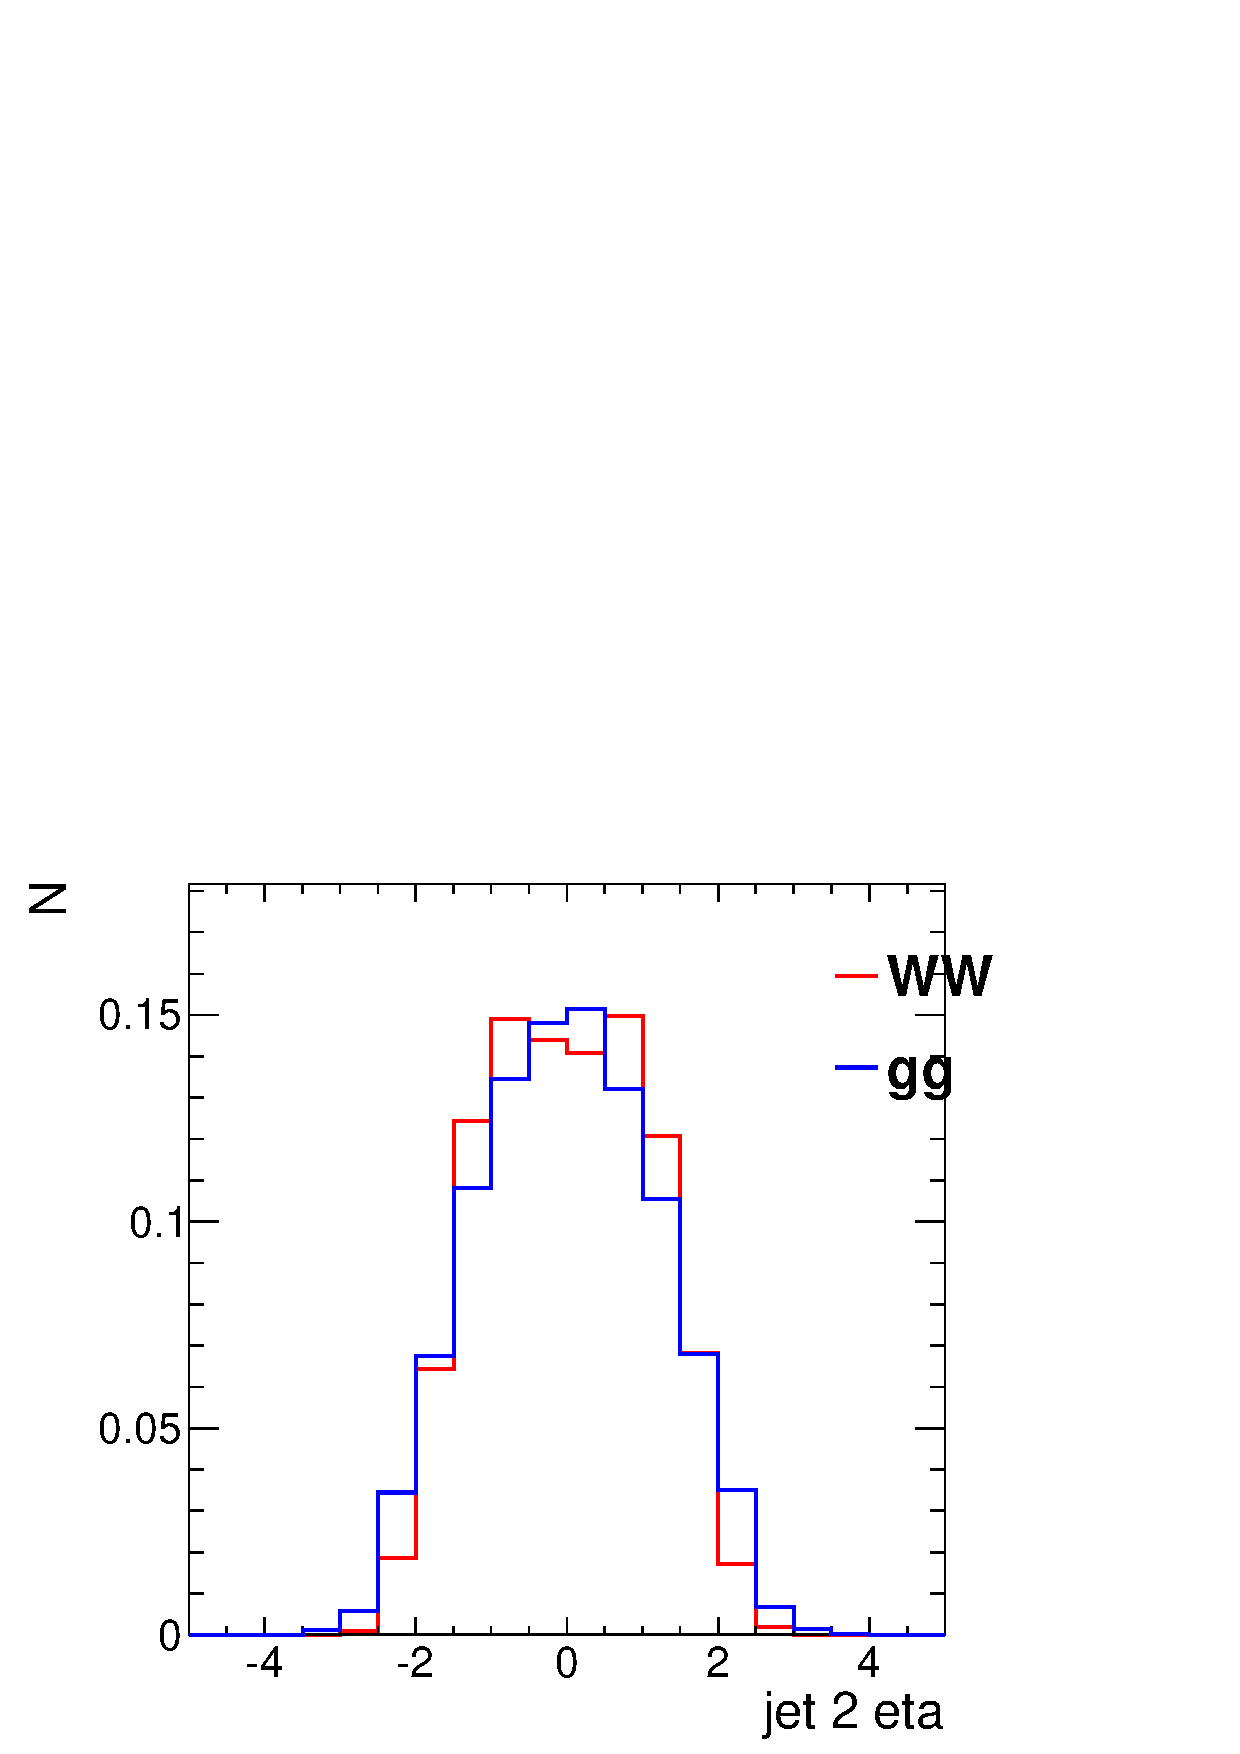
\includegraphics[width=0.48\textwidth]{./Figures/WTagging/pT500/AKtR08/jeta2.png}}
\caption{Comparisons of the QCD background to the WW signal in the \pt 500 GeV bin using the anti-\kT R=0.8 algorithm: basic
  kinematic distributons.}
\label{fig:pt500_basics_AKt_R08}
\end{center}
\end{figure*}


\subsection{Performance at Moderate Boosts}

(this section is to cover the $W$-tagging performance for jet \pT 200-300 GeV and
500-600 GeV using $\sqrt{s} = 8$ TeV samples)

\subsubsection{Single Variable Performance}

{\it Show plots of signal versus background for all single variables investigated}.

Figure~\ref{fig:pt500_mass_AKt_R08} the compares signal and background
 in the mass distributions for the different groomers, and Figure~\ref{fig:pt500_subst_AKt_R08}
in the different substructure variables. 

\begin{figure*}
\begin{center}
\subfigure[Ungroomed mass]{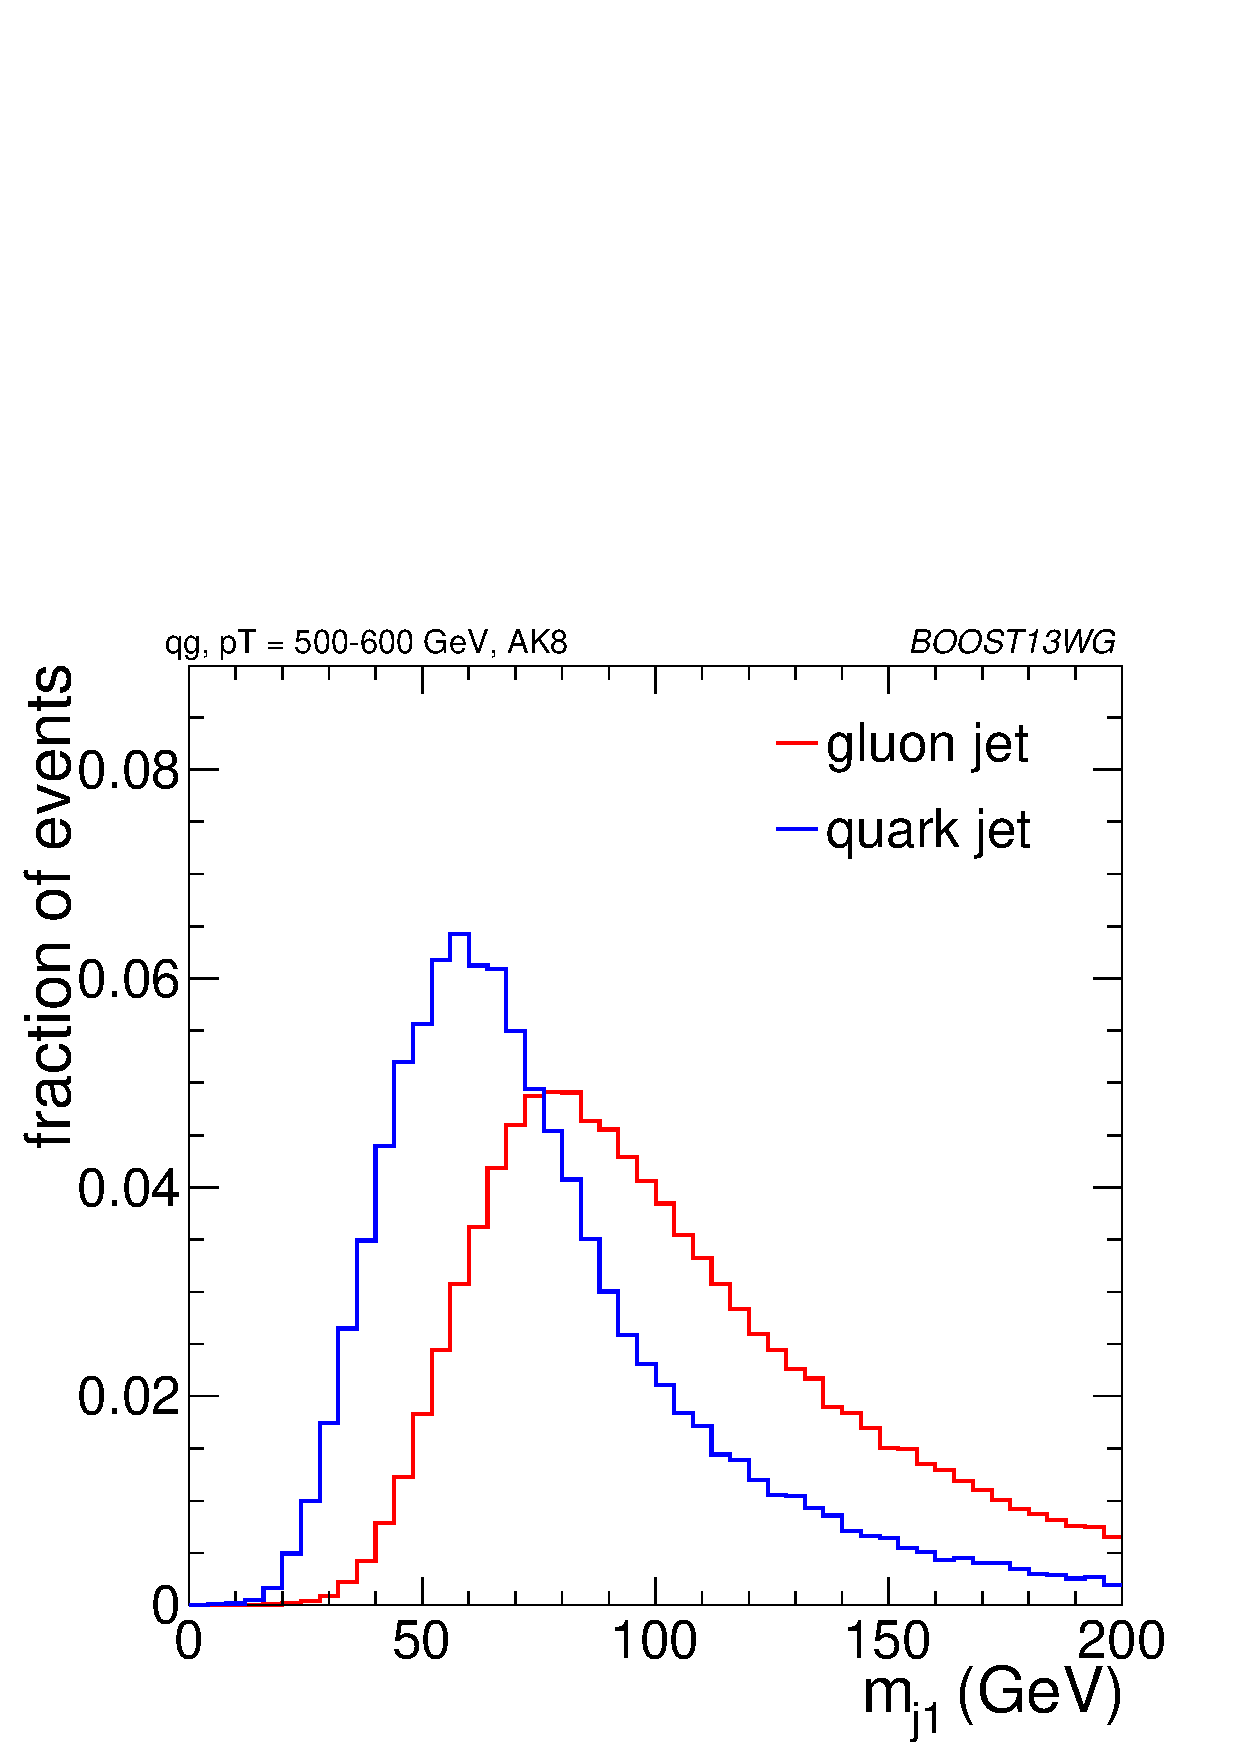
\includegraphics[width=0.48\textwidth]{./Figures/WTagging/pT500/AKtR08/jmass1.png}}
\subfigure[Pruned mass]{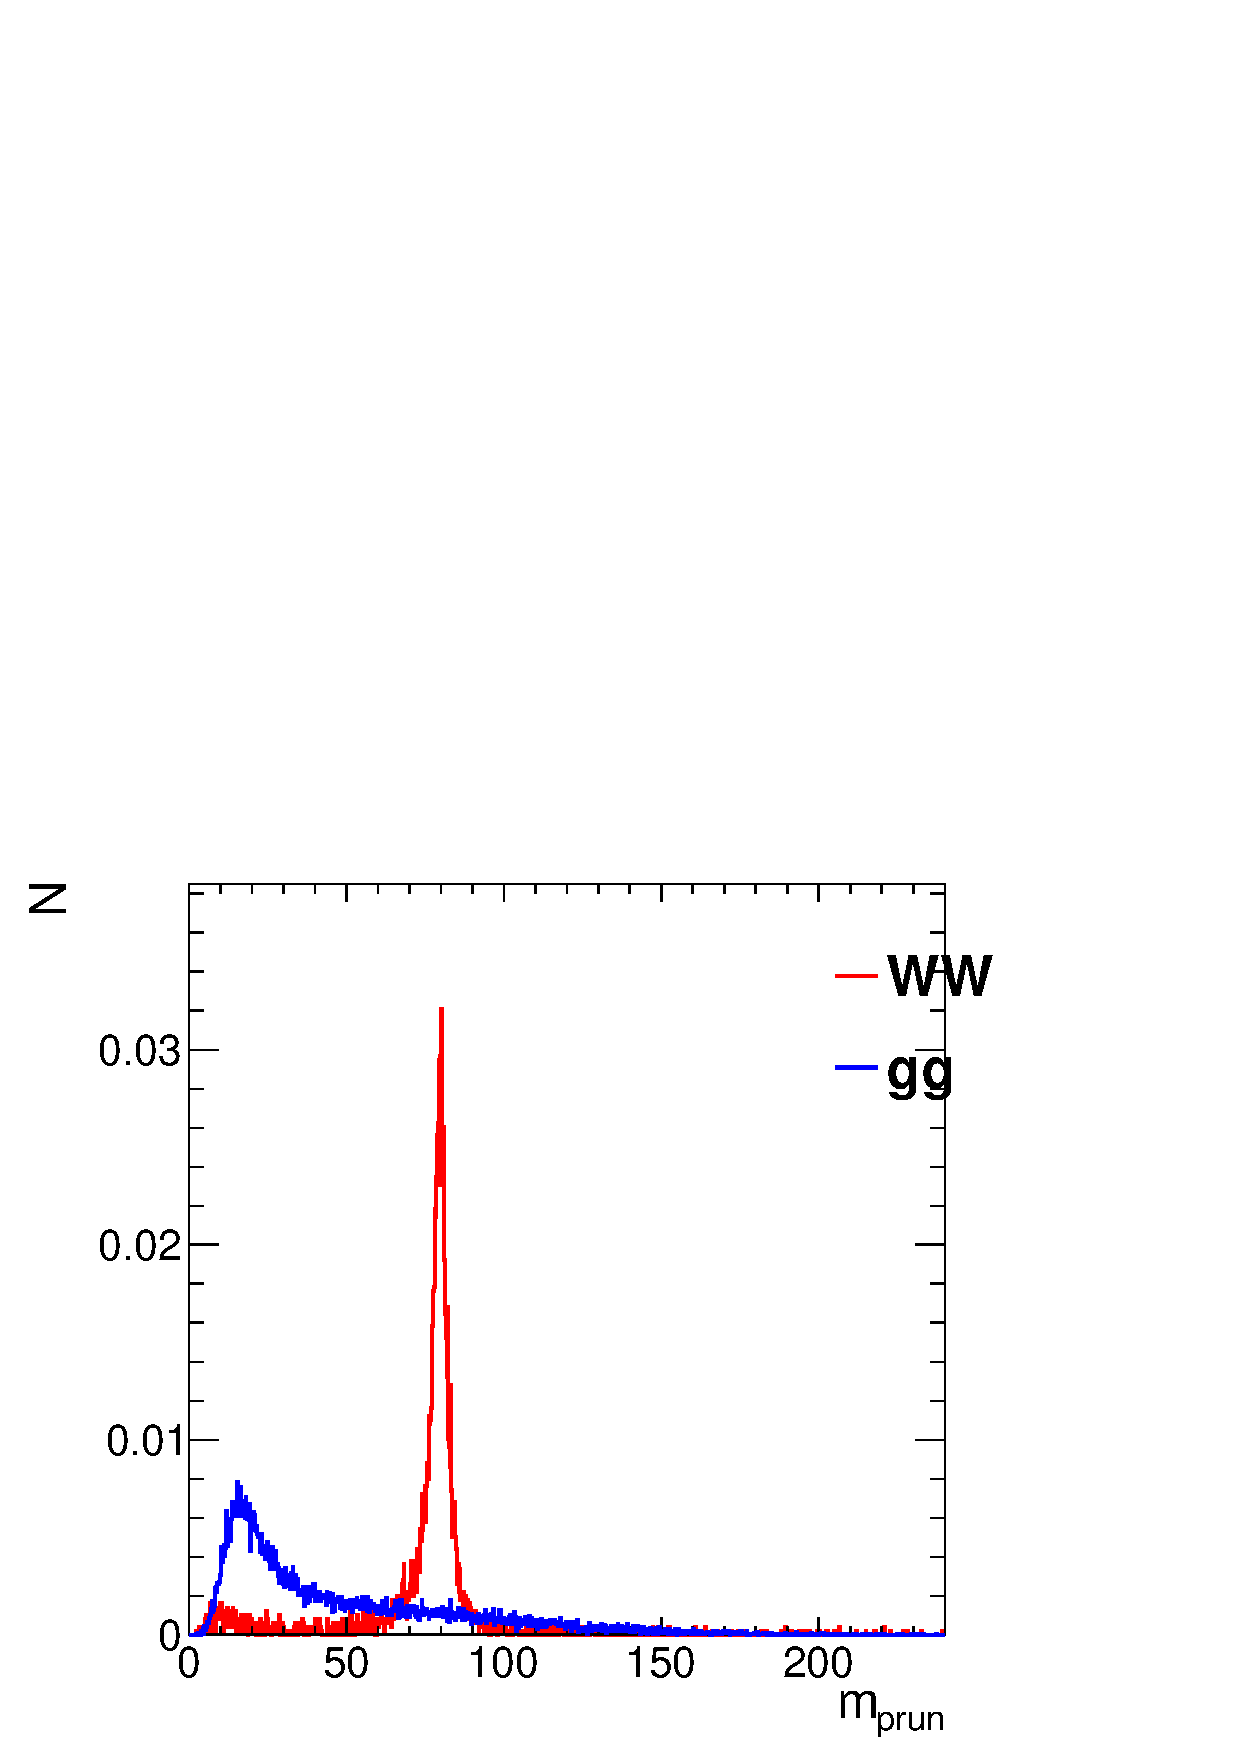
\includegraphics[width=0.48\textwidth]{./Figures/WTagging/pT500/AKtR08/h_mass_prun.png}}
\subfigure[Trimmed mass]{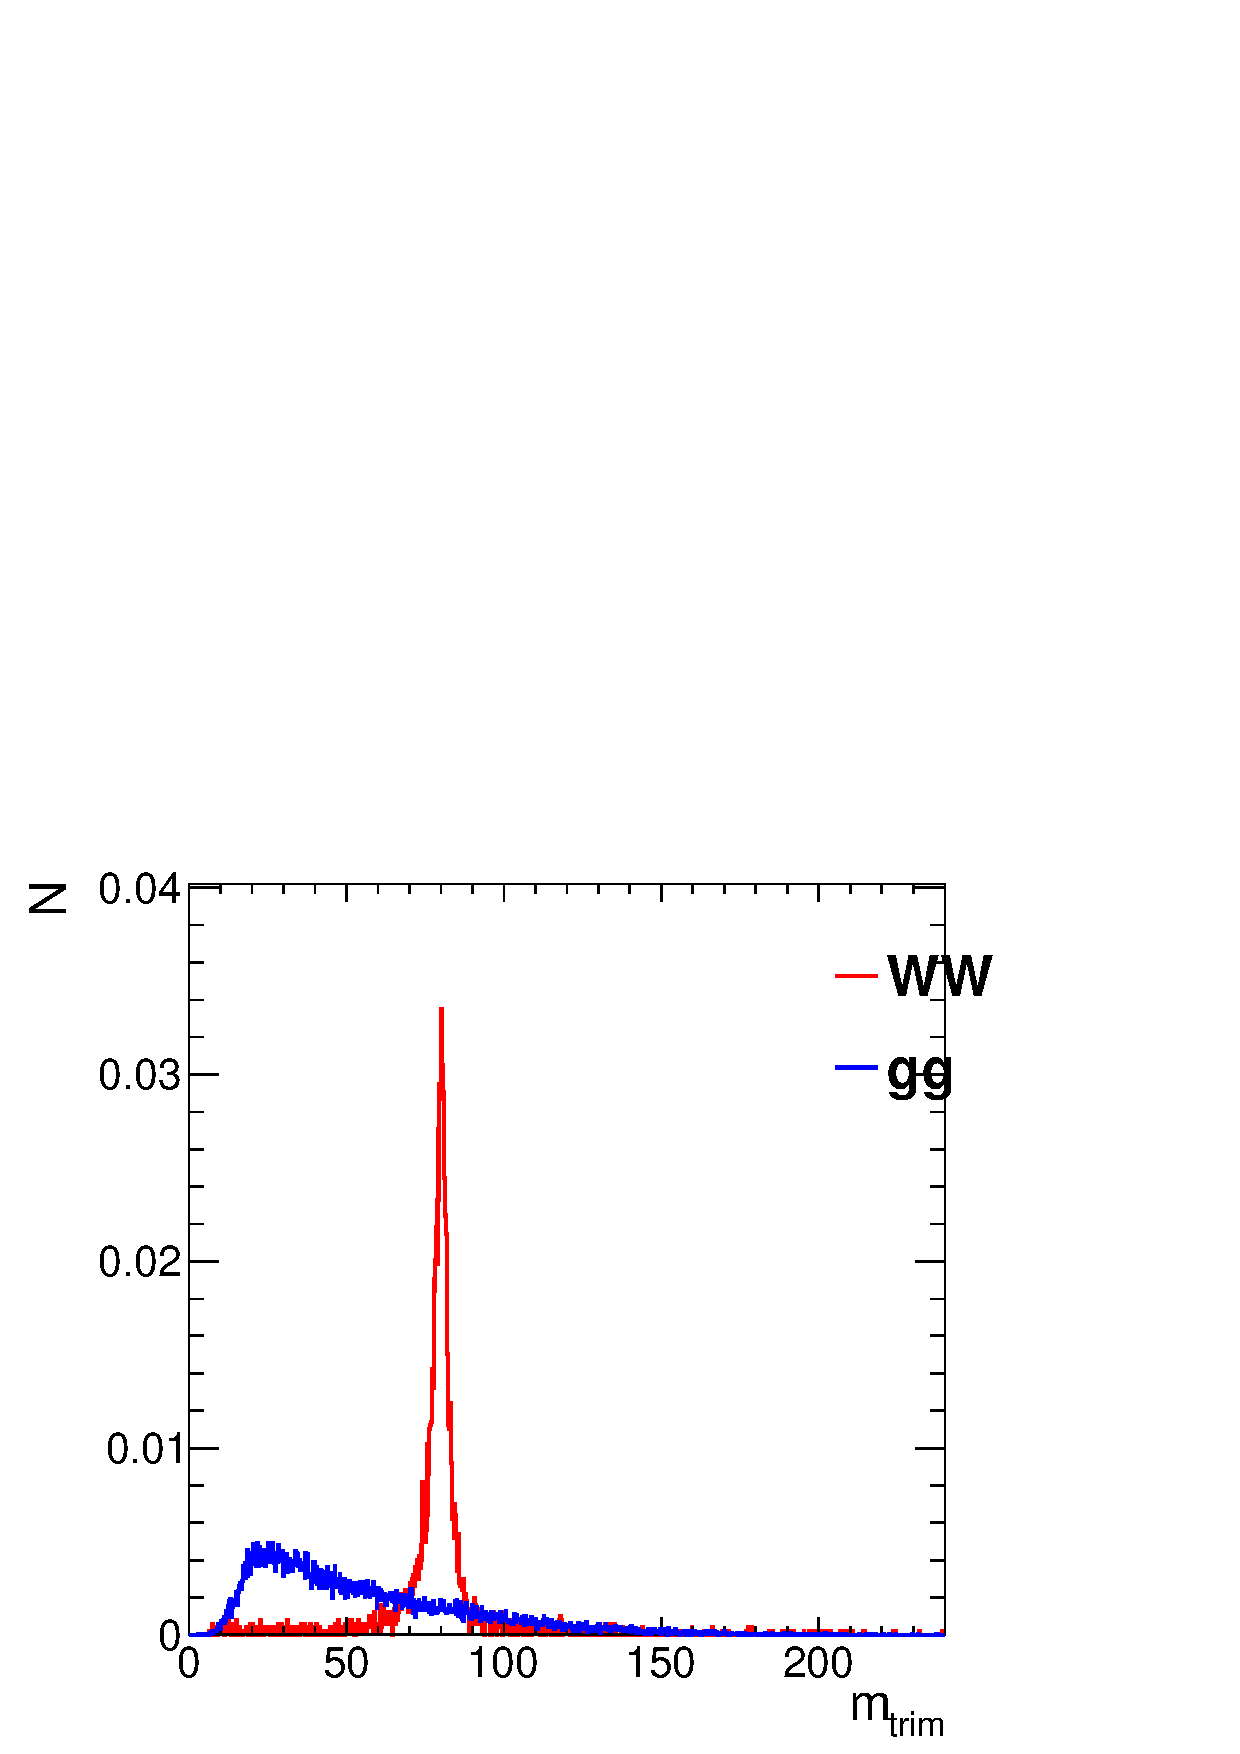
\includegraphics[width=0.48\textwidth]{./Figures/WTagging/pT500/AKtR08/h_mass_trim.png}}
\subfigure[mMDT mass]{\includegraphics[width=0.48\textwidth]{./Figures/WTagging/pT500/AKtR08/h_mass_mmdt.png}}
\subfigure[Soft-drop $\beta=2$ mass]{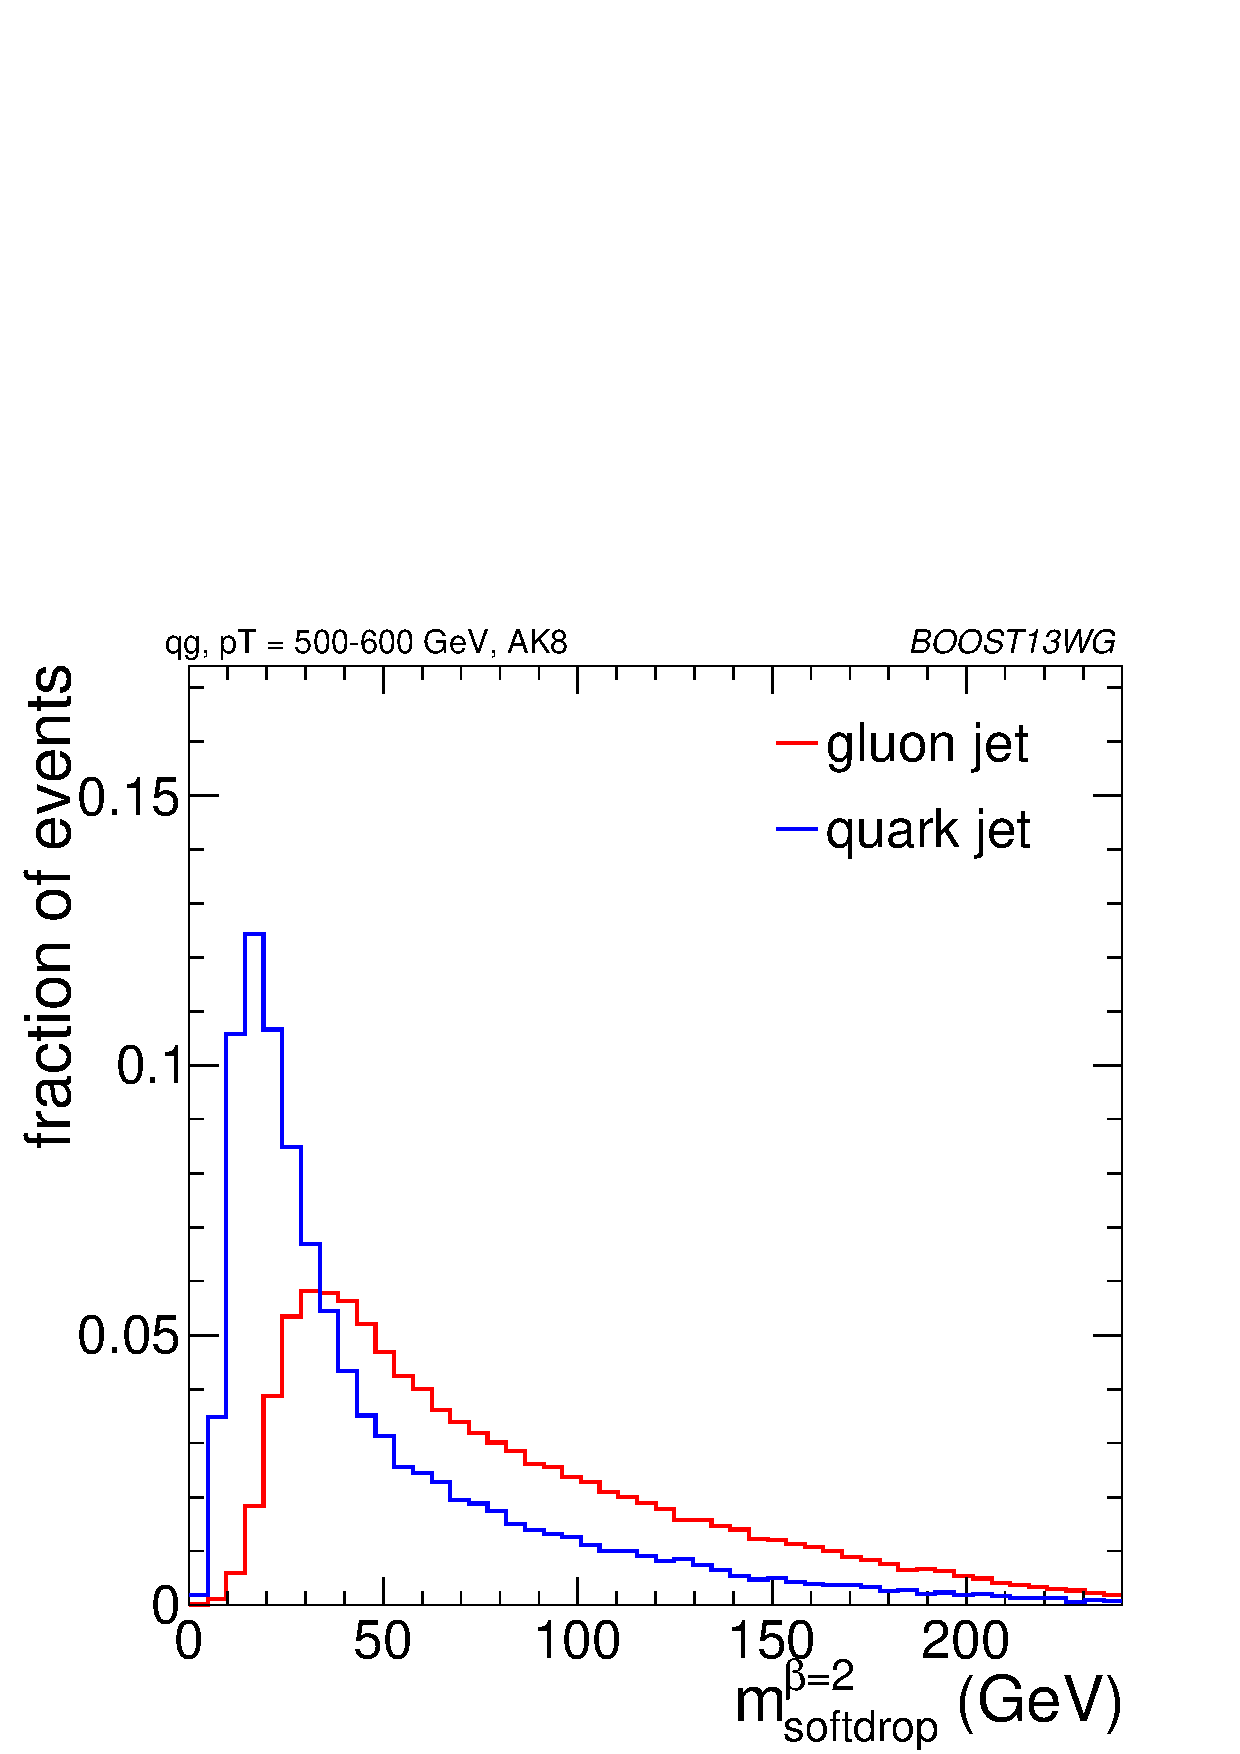
\includegraphics[width=0.48\textwidth]{./Figures/WTagging/pT500/AKtR08/h_mass_sdb2.png}}
\subfigure[Soft-drop $\beta=-1$ mass]{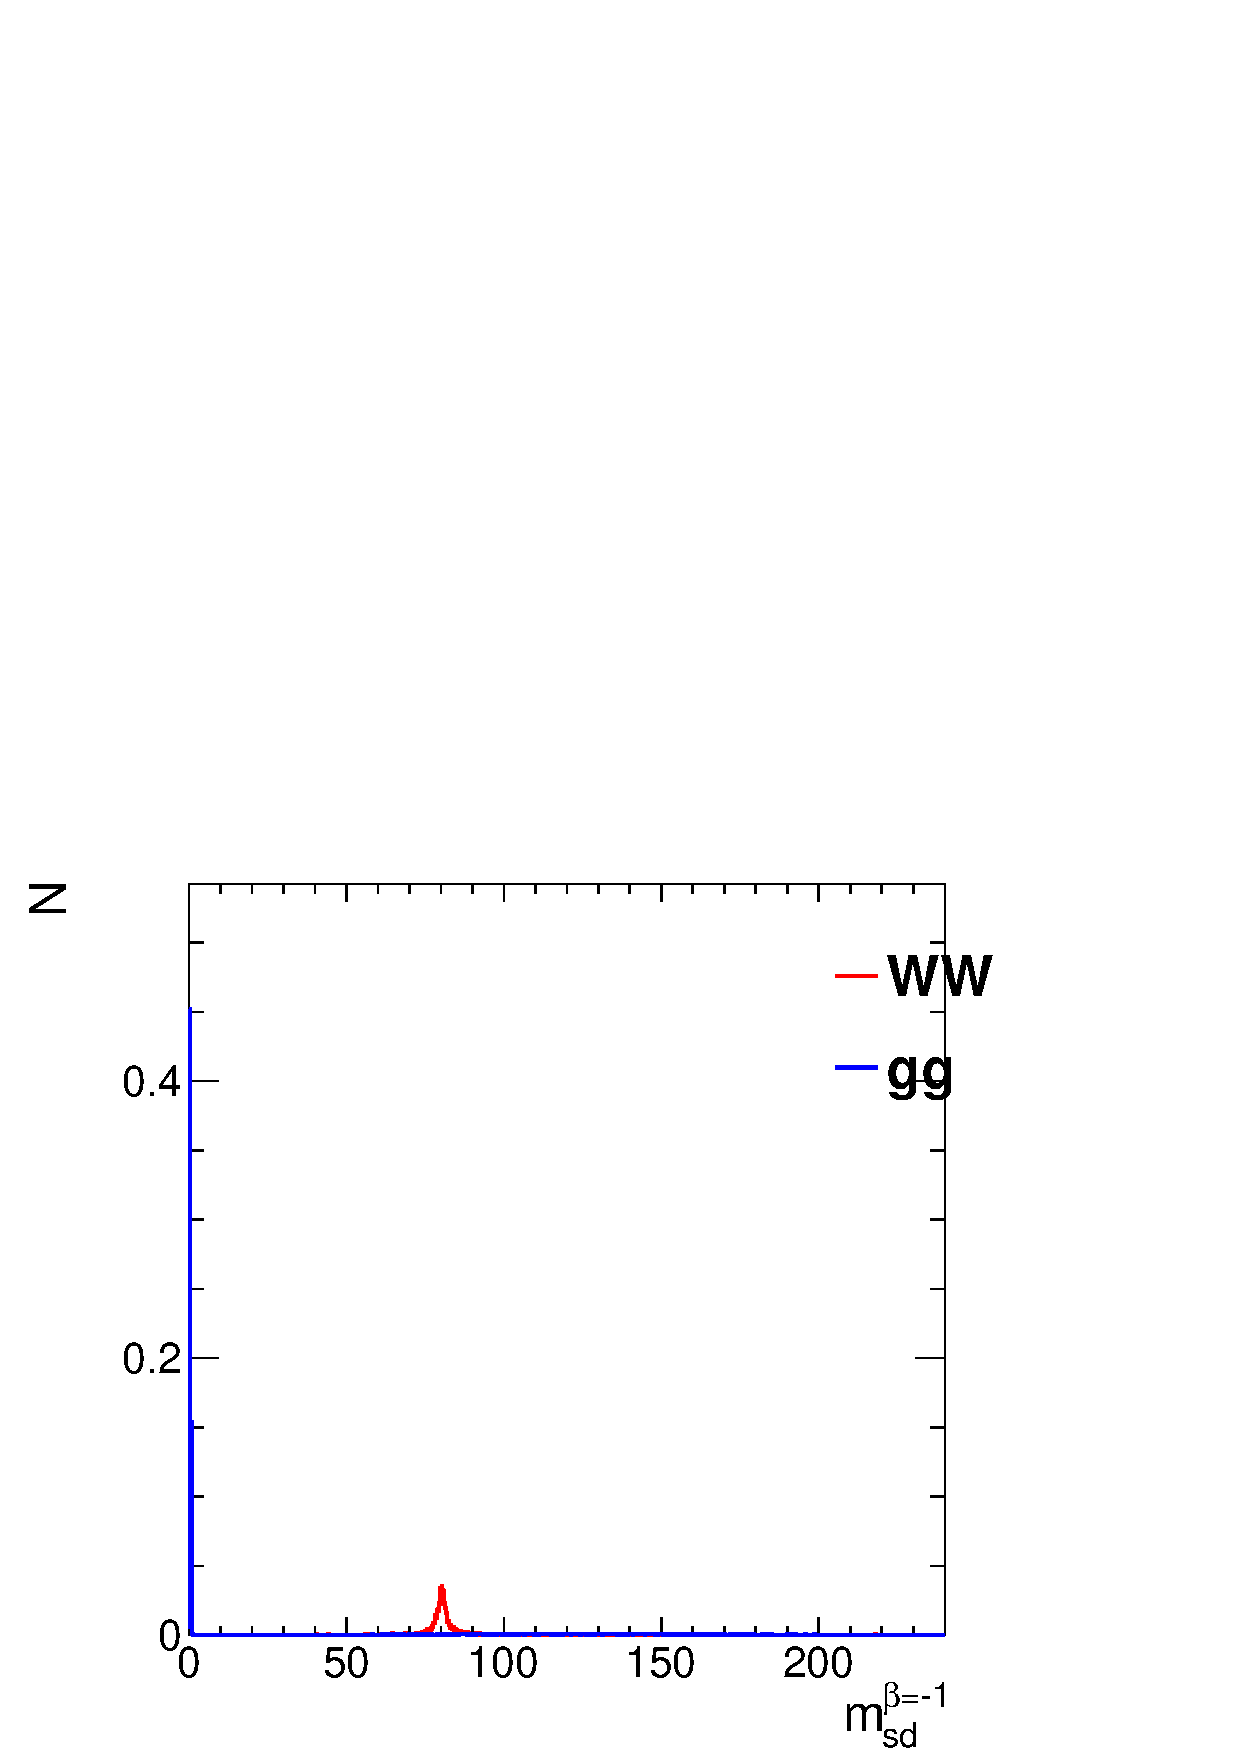
\includegraphics[width=0.48\textwidth]{./Figures/WTagging/pT500/AKtR08/h_mass_sdm1.png}}
\caption{Comparisons of the QCD background to the WW signal in the \pt 500 GeV bin using the anti-\kT R=0.8 algorithm: leading
  jet mass distributions.}
\label{fig:pt500_mass_AKt_R08}
\end{center}
\end{figure*}

\begin{figure*}
\begin{center}
\subfigure[$C_2^{\beta=1}$]{\includegraphics[width=0.48\textwidth]{./Figures/WTagging/pT500/AKtR08/h_c2_b1.png}}
\subfigure[$C_2^{\beta=2}$]{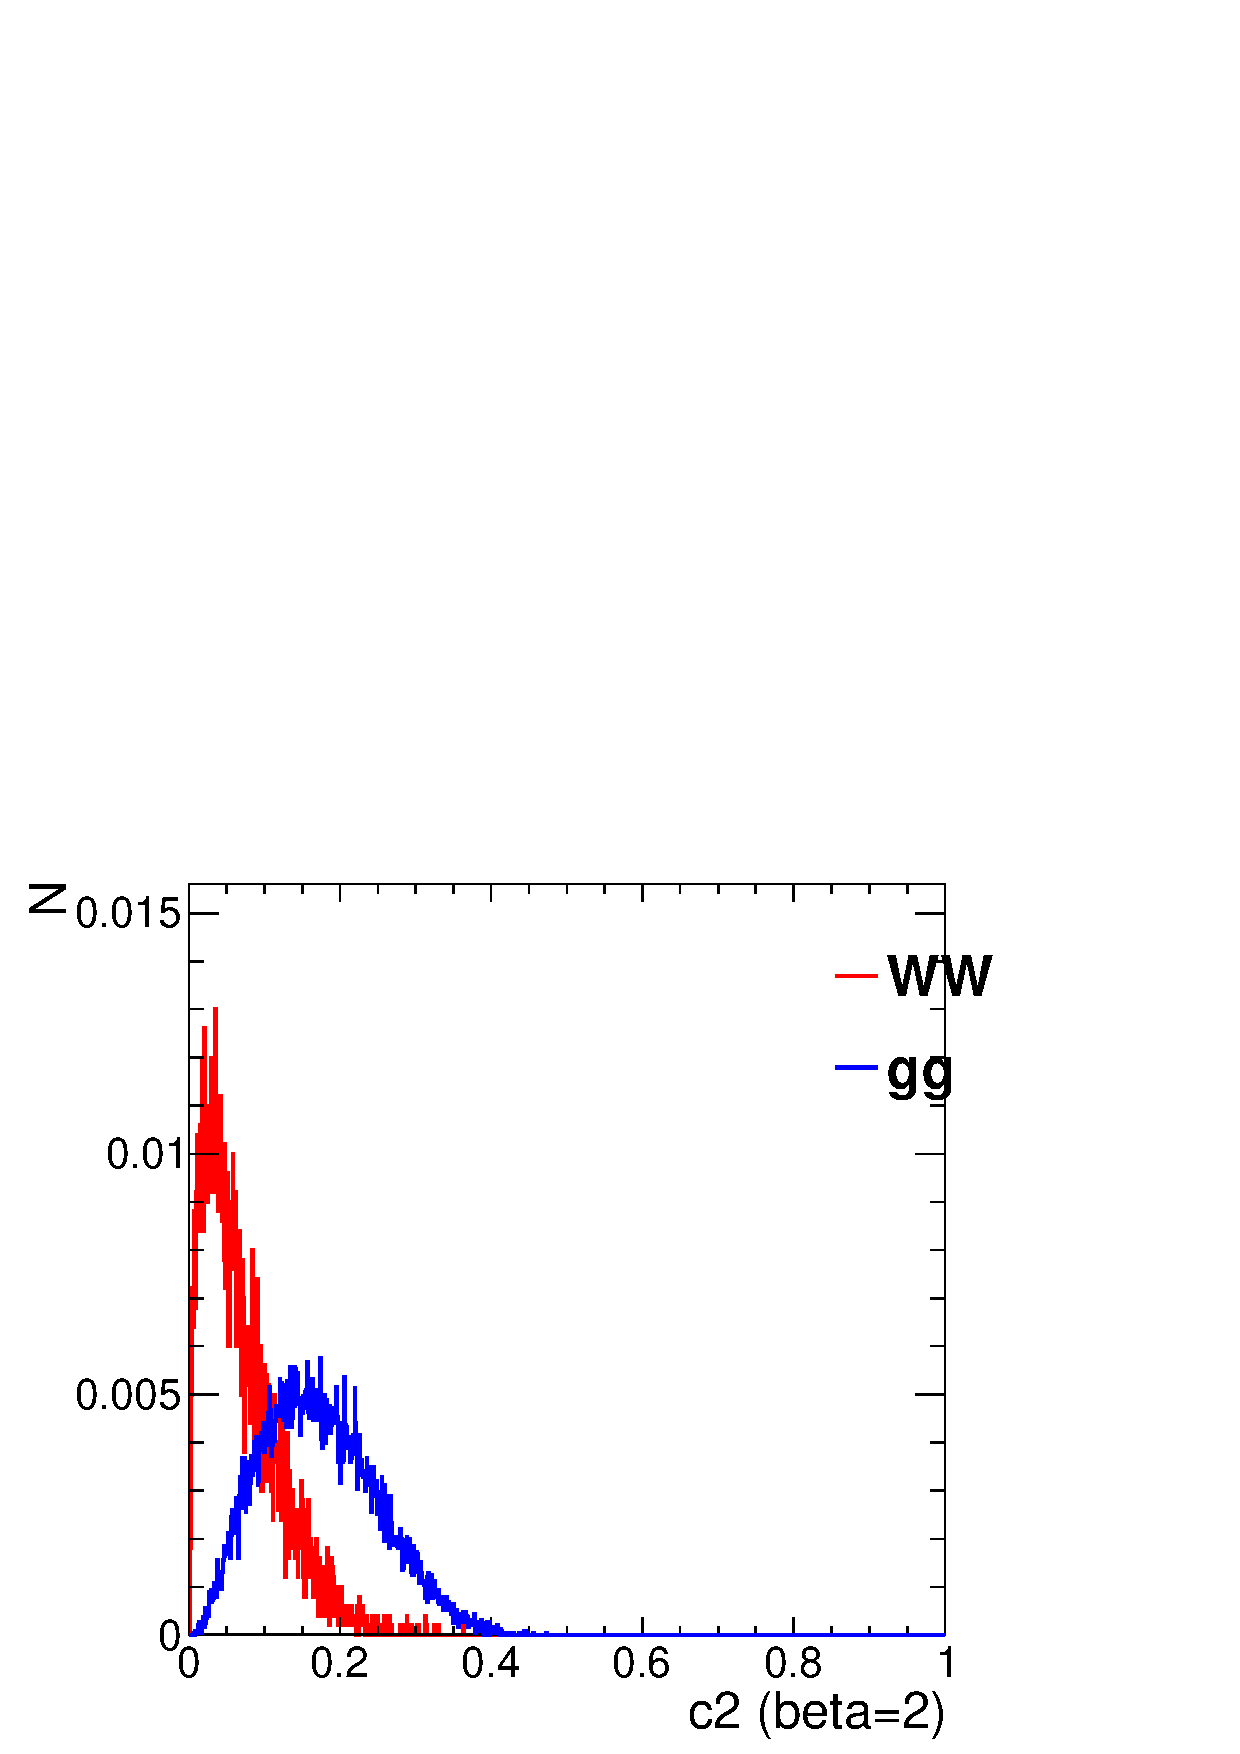
\includegraphics[width=0.48\textwidth]{./Figures/WTagging/pT500/AKtR08/h_c2_b2.png}}
\subfigure[$\Gamma_{Qjet}$]{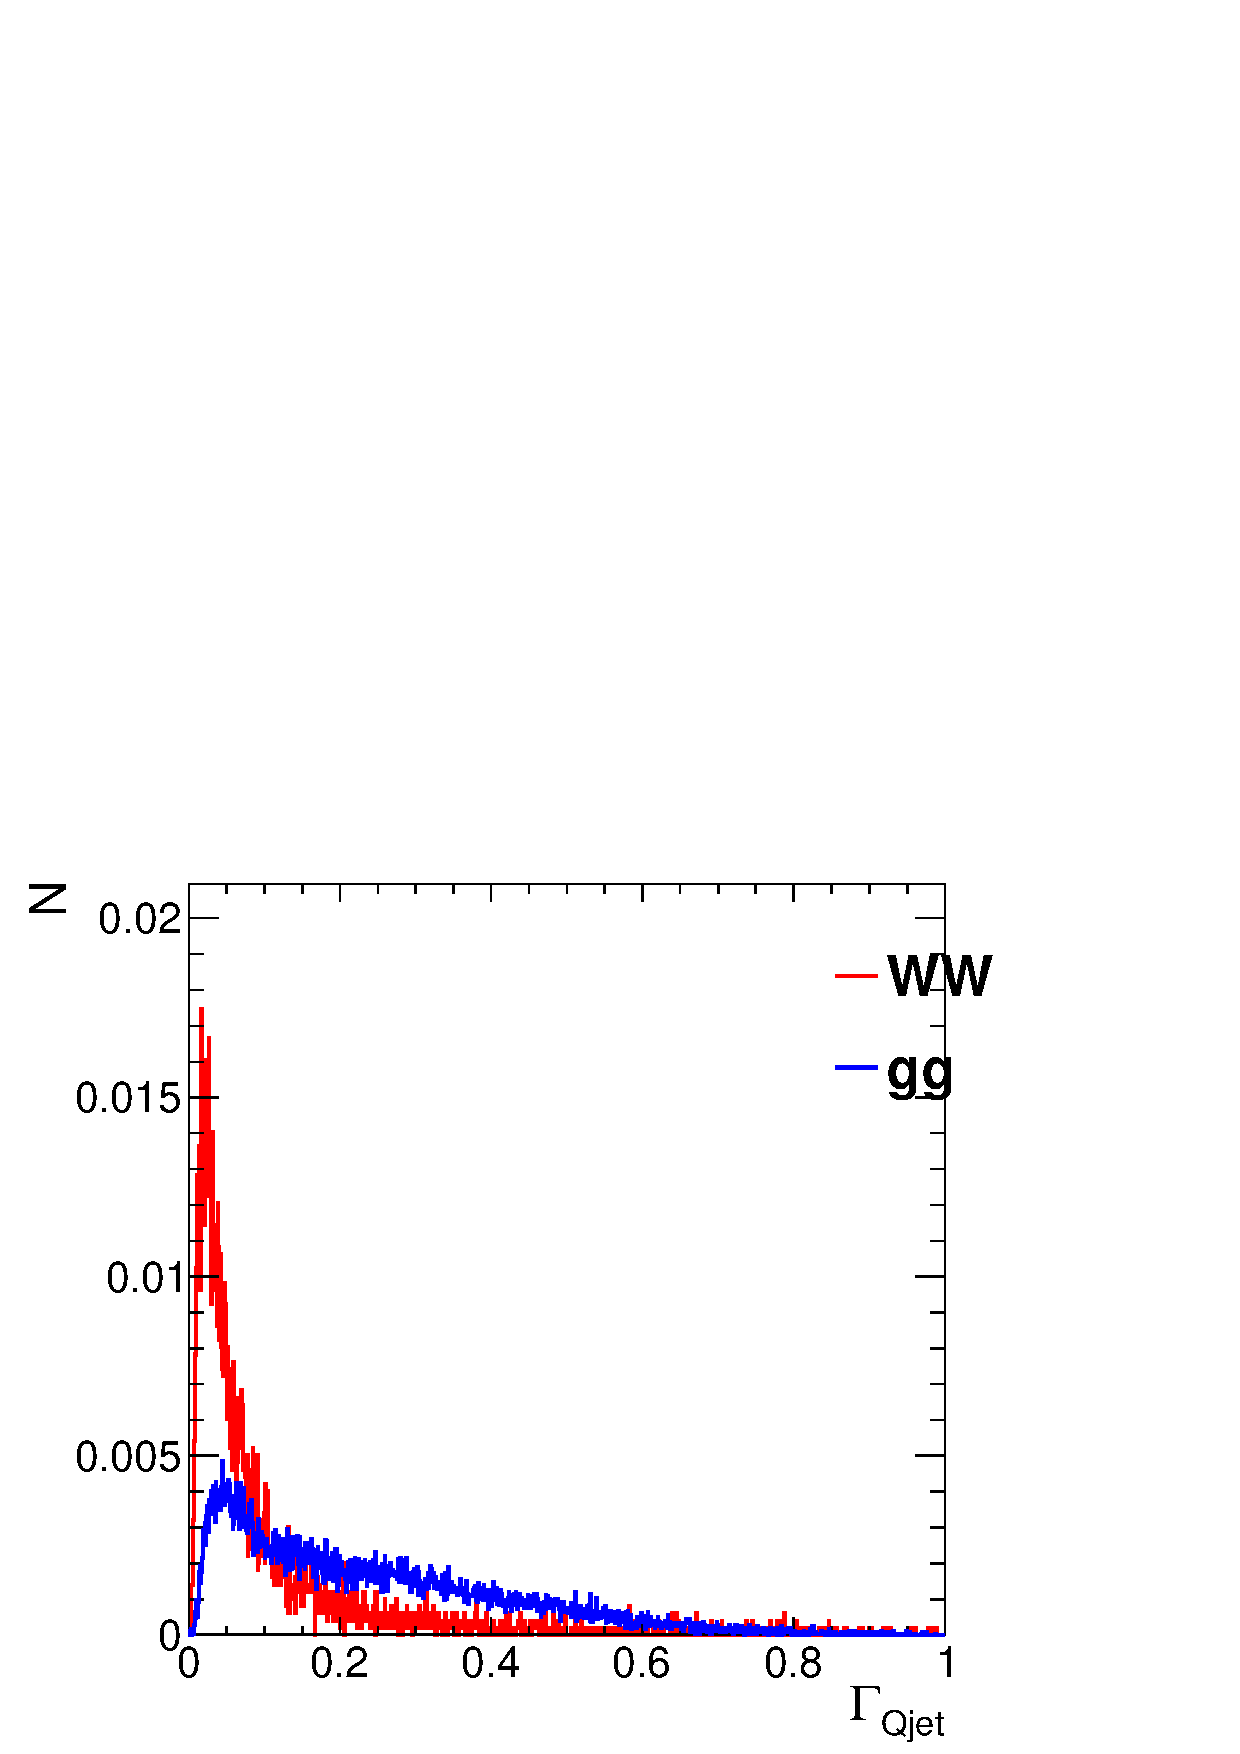
\includegraphics[width=0.48\textwidth]{./Figures/WTagging/pT500/AKtR08/h_qjetVol.png}}
\subfigure[$\tau_{21}^{\beta=1}$]{\includegraphics[width=0.48\textwidth]{./Figures/WTagging/pT500/AKtR08/h_tau21_b1.png}}
\subfigure[$\tau_{21}^{\beta=2}$]{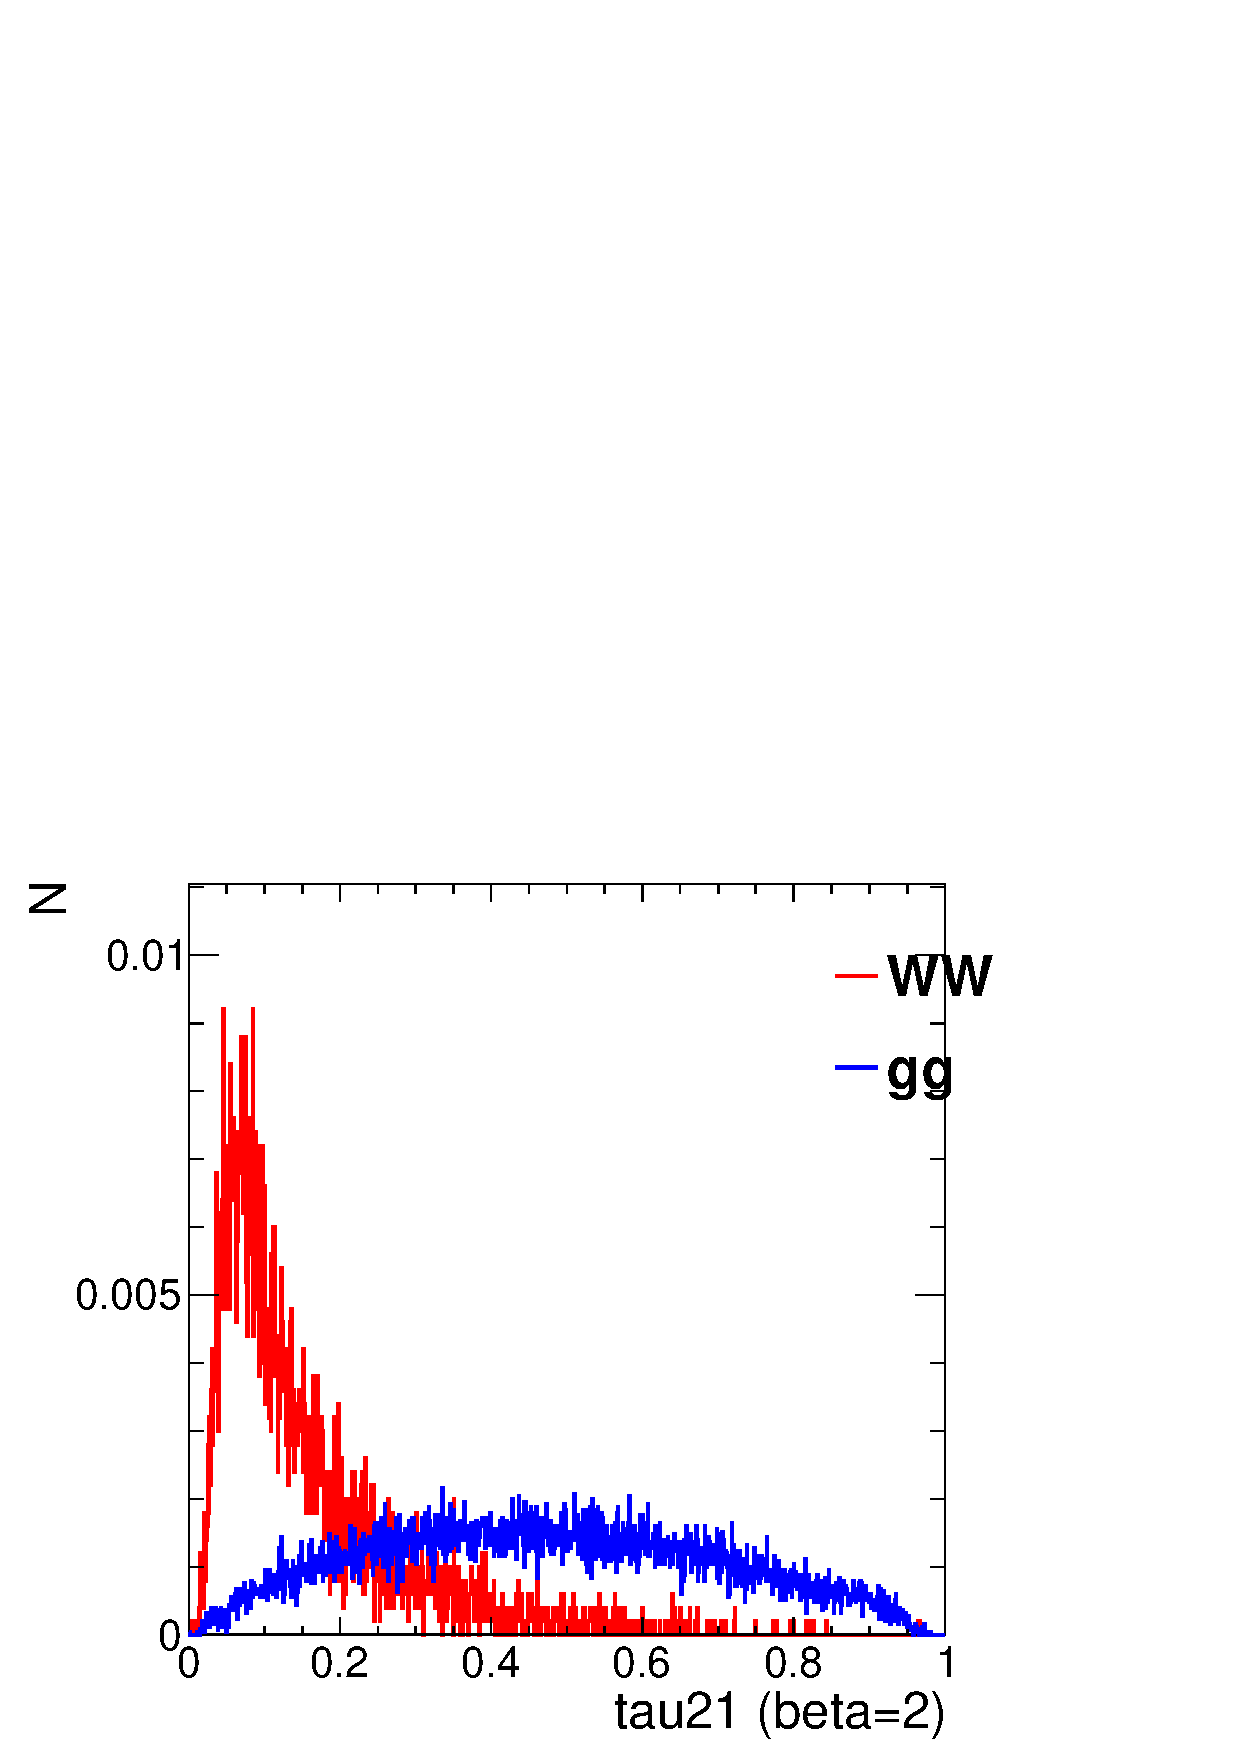
\includegraphics[width=0.48\textwidth]{./Figures/WTagging/pT500/AKtR08/h_tau21_b2.png}}
\caption{Comparisons of the QCD background to the WW signal in the \pt 500 GeV bin using the anti-\kT R=0.8 algorithm:
  substructure variables.}
\label{fig:pt500_subst_AKt_R08}
\end{center}
\end{figure*}


Figure~\ref{fig:pt500_single_AKt_R08} shows the single variable ROC curves in
the \pT 500 GeV bin for the anti-\kT R=0.8 algorithm, compared to the
ROC curve for a BDT combination of all the variables. One can see that
the best performant single variables for a reasonable signal
efficiency are the groomed/filtered masses, which all have a similar
level of performance with the exception of the soft drop mass with $\beta=-1$. {\it Would be good to split this into two plots, one
using the masses and one for other variables, or somehow make the mass
and other variable curves more distinct from one another by using same
colour for all the mass curves}.

{\it We want to look also at:
\begin{itemize}
\item Dependence on R. So have the same single variable ROC for
e.g. R=1.2, R=0.4. Then possibly have another plot which compares the
best single variable (e.g. groomed mass) for
different R.
\item Dependence on pT. Again want to repeat the plot for different
kinematic bins, and then have a plot which compares the best
performance in each kinematic bin to see the dependence of performance
on kinematics.
\end{itemize}
}

\begin{figure*}
\begin{center}
\includegraphics[width=0.8\textwidth]{./Figures/WTagging/pT500/AKtR08/Rocs_1D_single.png}
\caption{The ROC curve for all single variables considered for $W$
tagging in the \pt 500 GeV bin using the anti-\kT R=0.8 algorithm.}
\label{fig:pt500_single_AKt_R08}
\end{center}
\end{figure*}

Figure~\ref{fig:pt500_single_AKt_R12} shows the single variable ROC curves in
the \pT 500 GeV bin for the anti-\kT R=1.2 algorithm, compared to the
ROC curve for a BDT combination of all the variables. Comparing to
Figure~\ref{fig:pt500_single_AKt_R08}, one can see that the
performance of the groomed masses is quite similar. However, the
performance of the other non-mass substructure variables is markedly
different, and better in the R=0.8 case.

\begin{figure*}
\begin{center}
\includegraphics[width=0.8\textwidth]{./Figures/WTagging/pT500/AKtR12/Rocs_1D_single.png}
\caption{The ROC curve for all single variables considered for $W$
tagging in the \pt 500 GeV bin using the anti-\kT R=1.2 algorithm.}
\label{fig:pt500_single_AKt_R12}
\end{center}
\end{figure*}


\subsubsection{Combined Performance}

\subsubsection*{Mass + X Performance}

Figure~\ref{fig:pt500_masscomb_AKt_R08} shows the BDT combinations of each mass variable with every other
variable considered in the \pt 500 GeV bin using the anti-\kT R=0.8
algorithm. {\it Can we drop the combinations of mass + mass
from these plots to make them clearer? Also would be good to put the
single variable mass curve on these plots, so you can see how much
improvement the combination gives, and the ``all variables'' curve.}

No combination with other variables can recover the poor performance
of the ungroomed mass and the soft drop mass with $\beta=-1$. The
other groomed/filtered masses are all most improved by combination
with the $C_{2}^{\beta=1}$ energy correlation
function. Figure~\ref{fig:pt500_2d_mmdt_AKt_R08} shows the 2-D
correlation plots between the mMDT mass and the $C_{2}^{\beta=1}$,
$\Gamma_{Qjet}$ and $\tau_{21}^{\beta=1}$ variables. One can clearly
see that there is substantially less correlation between the mass and
$C_{2}^{\beta=1}$ than the other variables. Similar results are seen
for the other groomed masses.

\begin{figure*}
\begin{center}
\subfigure[Ungroomed mass + X]{\includegraphics[width=0.48\textwidth]{./Figures/WTagging/pT500/AKtR08/Rocs_1D_jmass.png}}
\subfigure[Trimmed mass + X]{\includegraphics[width=0.48\textwidth]{./Figures/WTagging/pT500/AKtR08/Rocs_1D_j_mass_trim.png}}
\subfigure[Pruned mass + X]{\includegraphics[width=0.48\textwidth]{./Figures/WTagging/pT500/AKtR08/Rocs_1D_j_mass_prun.png}}
\subfigure[Soft drop mass ($\beta=-1$) +X]{\includegraphics[width=0.48\textwidth]{./Figures/WTagging/pT500/AKtR08/Rocs_1D_j_mass_sdm1.png}}
\subfigure[Soft drop mass ($\beta=2$) + X]{\includegraphics[width=0.48\textwidth]{./Figures/WTagging/pT500/AKtR08/Rocs_1D_j_mass_sdb2.png}}
\subfigure[mMDT mass + X]{\includegraphics[width=0.48\textwidth]{./Figures/WTagging/pT500/AKtR08/Rocs_1D_j_mass_mmdt.png}}
\caption{The BDT combinations of each mass variable with every other
variable considered in the \pt 500 GeV bin using the anti-\kT R=0.8 algorithm.}
\label{fig:pt500_masscomb_AKt_R08}
\end{center}
\end{figure*}

\begin{figure*}
\begin{center}
\subfigure[mMDT mass vs $C_2^{\beta=1}$]{\includegraphics[width=0.48\textwidth]{./Figures/WTagging/pT500/AKtR08/h2d_jc2_b1_j_mass_mmdt_gg.png}}
\subfigure[mMDT mass vs $\Gamma_{Qjet}$]{\includegraphics[width=0.48\textwidth]{./Figures/WTagging/pT500/AKtR08/h2d_j_qjetVol_j_mass_mmdt_gg.png}}
\subfigure[mMDT mass vs $\tau_{21}^{\beta=1}$]{\includegraphics[width=0.48\textwidth]{./Figures/WTagging/pT500/AKtR08/h2d_jtau21_b1_j_mass_mmdt_gg.png}}
\caption{2-D plots showing the correlation between mMDT mass and
  various substructure variables in the \pt 500 GeV bin using the
  anti-\kT R=0.8 algorithm in the gg sample.}
\label{fig:pt500_2d_mmdt_AKt_R08}
\end{center}
\end{figure*}

Figure~\ref{fig:pt500_masscomb_AKt_R12} shows the BDT combinations of
the bset performant groomed masses with every other
variable considered in the \pt 500 GeV bin using the anti-\kT R=1.2
algorithm. Interestingly, the groomed masses are now all most improved by combination
with the $\tau_{21}^{\beta=1}$ variable, in contrast with
$C_{2}^{\beta=1}$ which performed best for the smaller radius of
R=0.8. One can see from Figure~\ref{fig:pt500_single_AKt_R12} that the
single variable discrimination of $\tau_{21}^{\beta=1}$ and
$C_{2}^{\beta=1}$ changes quite markedly when the distance parameter R
is varied, although in both cases $C_{2}^{\beta=1}$ is a better single
variable discriminant (except for very high signal
efficiencies). Figure~\ref{fig:pt500_subst_AKt_R08_R12} shows how the
actual distributions of the $C_{2}^{\beta=1}$ and $\tau_{21}^{\beta=1}$
change when we change the distance parameter. Figure~\ref{fig:pt500_2d_mmdt_AKt_R12} shows the 2-D
correlation plots between between the mMDT mass and the $C_{2}^{\beta=1}$,
$\Gamma_{Qjet}$ and $\tau_{21}^{\beta=1}$ variables for the R=1.2
case. It is hard to see a substantial difference in the correlations
here versus Figure~\ref{fig:pt500_2d_mmdt_AKt_R08}, but perhaps
$C_{2}^{\beta=1}$ is marginally more correlated with the mass for
R=1.2 compared to R=0.8.

\begin{figure*}
\begin{center}
\subfigure[$C_2^{\beta=1}$, R=0.8]{\includegraphics[width=0.48\textwidth]{./Figures/WTagging/pT500/AKtR08/h_c2_b1.png}}
\subfigure[$C_2^{\beta=1}$, R=1.2]{\includegraphics[width=0.48\textwidth]{./Figures/WTagging/pT500/AKtR12/h_c2_b1.png}}
\subfigure[$\tau_{21}^{\beta=1}$, R=0.8]{\includegraphics[width=0.48\textwidth]{./Figures/WTagging/pT500/AKtR08/h_tau21_b1.png}}
\subfigure[$\tau_{21}^{\beta=1}$, R=1.2]{\includegraphics[width=0.48\textwidth]{./Figures/WTagging/pT500/AKtR12/h_tau21_b1.png}}
\caption{Comparisons of the QCD background to the WW signal in the \pt
  500 GeV bin for $C_2^{\beta=1}$ and $\tau_{21}^{\beta=1}$ variables
  and using the R=0.8 and R=1.2 anti-\kT distance parameters.}
\label{fig:pt500_subst_AKt_R08_R12}
\end{center}
\end{figure*}

{\it Now show a plot which compares on one plot the best combined performance for
each groomed mass + X for both R=0.8 and 1.2 cases e.g. mass +
$C_{2}^{\beta=1}$ for R=0.8 and mass + $\tau_{21}^{\beta=1}$ for R=1.2,
  and draw on also the
all variables curve for both R=0.8,1.2. 
Then we can see if there is much dependence on choice of mass once you
combine with another variable, and compare directly the two distance parameters.
This plot is just for
one kinematic bin, we should make the same plot for others.}

{\it Repeat these studies for different R and different kinematic
bins. Finally make plots which compare best combined performance for
different R and kinematics.}

{\it Do we want to look at other combinations of variables which don't
involve mass? Practically I think we will always be making mass + X though.}



\begin{figure*}
\begin{center}
%\subfigure[Ungroomed mass + X]{\includegraphics[width=0.48\textwidth]{./Figures/WTagging/pT500/AKtR12/Rocs_1D_jmass.png}}
\subfigure[Trimmed mass + X]{\includegraphics[width=0.48\textwidth]{./Figures/WTagging/pT500/AKtR12/Rocs_1D_j_mass_trim.png}}
\subfigure[Pruned mass + X]{\includegraphics[width=0.48\textwidth]{./Figures/WTagging/pT500/AKtR12/Rocs_1D_j_mass_prun.png}}
%\subfigure[Soft drop mass ($\beta=-1$) +X]{\includegraphics[width=0.48\textwidth]{./Figures/WTagging/pT500/AKtR12/Rocs_1D_j_mass_sdm1.png}}
\subfigure[Soft drop mass ($\beta=2$) + X]{\includegraphics[width=0.48\textwidth]{./Figures/WTagging/pT500/AKtR12/Rocs_1D_j_mass_sdb2.png}}
\subfigure[mMDT mass + X]{\includegraphics[width=0.48\textwidth]{./Figures/WTagging/pT500/AKtR12/Rocs_1D_j_mass_mmdt.png}}
\caption{The BDT combinations of each mass variable with every other
variable considered in the \pt 500 GeV bin using the anti-\kT R=1.2 algorithm.}
\label{fig:pt500_masscomb_AKt_R12}
\end{center}
\end{figure*}

\begin{figure*}
\begin{center}
\subfigure[mMDT mass vs $C_2^{\beta=1}$]{\includegraphics[width=0.48\textwidth]{./Figures/WTagging/pT500/AKtR12/h2d_jc2_b1_j_mass_mmdt_gg.png}}
\subfigure[mMDT mass vs $\Gamma_{Qjet}$]{\includegraphics[width=0.48\textwidth]{./Figures/WTagging/pT500/AKtR12/h2d_j_qjetVol_j_mass_mmdt_gg.png}}
\subfigure[mMDT mass vs $\tau_{21}^{\beta=1}$]{\includegraphics[width=0.48\textwidth]{./Figures/WTagging/pT500/AKtR12/h2d_jtau21_b1_j_mass_mmdt_gg.png}}
\caption{2-D plots showing the correlation between mMDT mass and
  various substructure variables in the \pt 500 GeV bin using the
  anti-\kT R=1.2 algorithm in the gg sample.}
\label{fig:pt500_2d_mmdt_AKt_R12}
\end{center}
\end{figure*}


\subsubsection*{Mass + Mass Performance}

It's interesting also to study and understand how the different
groomed masses relate to each other and how they are correlated.

Figures~\ref{fig:pt500_2d_massQQ_AKt_R08} and Figures~\ref{fig:pt500_2d_massGG_AKt_R08} shows 2-D correlation plots of
the different types of groomed mass in the \pt 500 GeV bin using the anti-\kT R=0.8
algorithm.

{\it Worth also showing some ROC curves for mass + mass combinations?}


\begin{table*}[htbp!]
\centering
%\setlength\fboxsep{0pt}
%\setlength\fboxrule{0.25pt}
\caption{Action of various groomers on the jet mass distribution in the different phase space regions.  For pruning, $a_\text{prune} = \zcut R_0$ and for trimming $a_\text{trim} = \sqrt{\zcut} R_\text{sub}$.}
\begin{tabular}{c|c|c|c|c} 
Action & Pruning & Trimming & mMDT & SD ($\beta > 0$) \\ \hline
$m>\sqrt{\zcut}R_0 p_T$  &  $-$ & $-$ &  $-$  & $-$ \\ \hline
\parbox[c][3em][c]{7em}{$m<\sqrt{\zcut}R_0 p_T$\\$m>a_x p_T$} & \parbox[c][3em][c]{6em}{cuts soft \& \\ soft-collinear}  & \parbox[c][3em][c]{6em}{cuts soft \& \\ soft-collinear} & \parbox[c][3em][c]{6em}{cuts soft \& \\ soft-collinear} & \parbox[c][5em][c]{7em}{cuts soft \& \\ partially ($\beta$) \\ on soft-collinear}  \\ \hline
$m<a_x p_T$ & \parbox[c][5em][c]{7em}{cuts partially \\ on both soft \& \\  soft-collinear}   &$-$ & \parbox[c][3em][c]{6em}{cuts soft \& \\ soft-collinear} & \parbox[c][5em][c]{7em}{cuts soft \& \\ partially ($\beta$) \\ on soft-collinear} 
\end{tabular}
\label{tab:boostedtoprates}
\end{table*}


\begin{figure*}
\begin{center}
\subfigure[Trimmed mass vs Soft drop mass ($\beta=2$)]{\includegraphics[width=0.48\textwidth]{./Figures/WTagging/pT500/AKtR08/WvsQ/h2d_j_mass_trim_j_mass_sdb2_WW_onSame.png}}
\subfigure[Trimmed mass vs Pruned mass]{\includegraphics[width=0.48\textwidth]{./Figures/WTagging/pT500/AKtR08/WvsQ/h2d_j_mass_trim_j_mass_prun_WW_onSame.png}}
\subfigure[Trimmed mass vs mMDT mass]{\includegraphics[width=0.48\textwidth]{./Figures/WTagging/pT500/AKtR08/WvsQ/h2d_j_mass_trim_j_mass_mmdt_WW_onSame.png}}
\subfigure[mMDT mass vs Soft drop mass ($\beta=2$)]{\includegraphics[width=0.48\textwidth]{./Figures/WTagging/pT500/AKtR08/WvsQ/h2d_j_mass_mmdt_j_mass_sdb2_WW_onSame.png}}
\subfigure[Pruned mass vs Soft drop mass ($\beta=2$)]{\includegraphics[width=0.48\textwidth]{./Figures/WTagging/pT500/AKtR08/WvsQ/h2d_j_mass_prun_j_mass_sdb2_WW_onSame.png}}
\subfigure[mMDT mass vs Pruned mass]{\includegraphics[width=0.48\textwidth]{./Figures/WTagging/pT500/AKtR08/WvsQ/h2d_j_mass_mmdt_j_mass_prun_WW_onSame.png}}
\caption{2-D plots showing the correlation between different types of
  groomed mass in the \pt 500 GeV bin using the anti-\kT R=0.8
  algorithm, separately for the jets in the $X \rightarrow WW$ sample and the
  jets in the quark-quark sample.}
\label{fig:pt500_2d_massQQ_AKt_R08}
\end{center}
\end{figure*}

\begin{figure*}
\begin{center}
\subfigure[Trimmed mass vs Soft drop mass ($\beta=2$)]{\includegraphics[width=0.48\textwidth]{./Figures/WTagging/pT500/AKtR08/WvsG/h2d_j_mass_trim_j_mass_sdb2_WW_onSame.png}}
\subfigure[Trimmed mass vs Pruned mass]{\includegraphics[width=0.48\textwidth]{./Figures/WTagging/pT500/AKtR08/WvsG/h2d_j_mass_trim_j_mass_prun_WW_onSame.png}}
\subfigure[Trimmed mass vs mMDT mass]{\includegraphics[width=0.48\textwidth]{./Figures/WTagging/pT500/AKtR08/WvsG/h2d_j_mass_trim_j_mass_mmdt_WW_onSame.png}}
\subfigure[mMDT mass vs Soft drop mass ($\beta=2$)]{\includegraphics[width=0.48\textwidth]{./Figures/WTagging/pT500/AKtR08/WvsG/h2d_j_mass_mmdt_j_mass_sdb2_WW_onSame.png}}
\subfigure[Pruned mass vs Soft drop mass ($\beta=2$)]{\includegraphics[width=0.48\textwidth]{./Figures/WTagging/pT500/AKtR08/WvsG/h2d_j_mass_prun_j_mass_sdb2_WW_onSame.png}}
\subfigure[mMDT mass vs Pruned mass]{\includegraphics[width=0.48\textwidth]{./Figures/WTagging/pT500/AKtR08/WvsG/h2d_j_mass_mmdt_j_mass_prun_WW_onSame.png}}
\caption{2-D plots showing the correlation between different types of
  groomed mass in the \pt 500 GeV bin using the anti-\kT R=0.8
  algorithm, separately for the jets in the $X \rightarrow WW$ sample and the
  jets in the gluon-gluon sample.}
\label{fig:pt500_2d_massGG_AKt_R08}
\end{center}
\end{figure*}


\subsection{Performance at High Boosts}

(this section is to cover the $W$-tagging performance for jet \pT 1-1.1 TeV and
$>$ 1.5 TeV using $\sqrt{s} = 14$ TeV samples)

{\it Maybe we don't need to divide into different medium/high boost sections.}




